\providecommand{\main}{..}
\documentclass[\main/main.tex]{subfiles}
\begin{document}

\chapter{Results}
\section{Reproducing the results}
Test were run on multiple datasets, all containing non-structured textual documents. All tests were run via the \href{https://github.com/LucaCappelletti94/zipf_classifier/blob/master/tests/test_classifier.py}{test.py} file, available in the github repository, with the following parameters:
\begin{description}
	\item[Seed] The random uniform generator used to split files, run Kmeans etc\ldots were initialized to \(1242\).
	\item[Training percentage] Of every dataset, \(70\%\) of the documents were used for training the classifier. The remaining \(30\%\) were used for testing. The split of the training and testing datasets was done selecting documents following an uniform random distribution initialized with the seed above.
	\item[Kmeans clusters \(k\)] For every test, \(10\) clusters were used.
	\item[Kmeans iterations] For every test \(300\) iterations were run before assuming convergence. Better results may be obtained with more iterations.
	\item[CURE representatives percentage] For every test \(10\%\) of the training points were used as representative points.
	\item[CURE distance percentage] For every test chosen representative points were moved \(20\%\) towards their respective centroids.
	\item[Stopwords] Two stopwords list were used: an italian one and an english one. These are available on the repository of the project for reproducibility reason, but are easily available online.
\end{description}

The complete dataset is available at the following url:

\url{https://mega.nz/#!XCI3iCiZ!EpBtedozqBivPcWYi8oAj6jx38LAJnUaNDfjvgzJi3I}.

The already trained classifiers are available at the following url:

\url{https://mega.nz/#!yLAR0CSI!4g6jNfTeTpoEbss3P4jmuJyvTvv0Wmtw1sZQydQS1Qs}.

\section{What are the diagrams representing}
\subsection{Precision varying with neighbors number}
This graph shows the precision on growing number of neighbors, meaning that the classification is weighted on the given \(n\) number of neighbors and their distances from the considered point. On the proposed datasets, a low number of neighbors yielded best results. The other graphs shown are relative to the best results obtained exploring the neighbor space, but all results are available in the repository documentation. \textit{Not all results were clearly possible to be included in this document as its size would increase a hundred fold.}

\subsection{ROC Curves}
The ROC curve, or receiver operating characteristic curve, is a graphical plot that illustrates the diagnostic ability of a binary classifier system as its discrimination threshold is varied. For each class in every dataset a ROC curve is drawn to compare each class with every other one.

\subsection{Confusion matrices}
A confusion matrix, also known as an error matrix, is a specific table layout that allows visualization of the performance of an algorithm. Each row of the Matrix represents the instances in a predicted class while each column represents the instances in an actual class.

\subsection{Truncated SVD reduction}
A simple dimensionality reduction to visualize high dimensional datasets in 2D.

\subsection{Most defining word clouds}
The most important coordinates in the clusters used to classify texts for a given class.

\subsection{Representatives points usage}
An enumeration of counters of usages of clusters to classify texts for a given class.

\clearpage
\section{Authors}
The ``authors'' dataset contains \(315\) texts from 3 authors: D. H. Lawrence, Mark Twain and Oscar Wilde. Each author has \(105\) documents.
\subsection{Precision varying with neighbors number}
\begin{figure}
	\includegraphics[width=0.4\textwidth]{precision_scores/authors.png}
	\caption{Precision scores}
\end{figure}
\subsection{ROC Curves}
\begin{figure}
	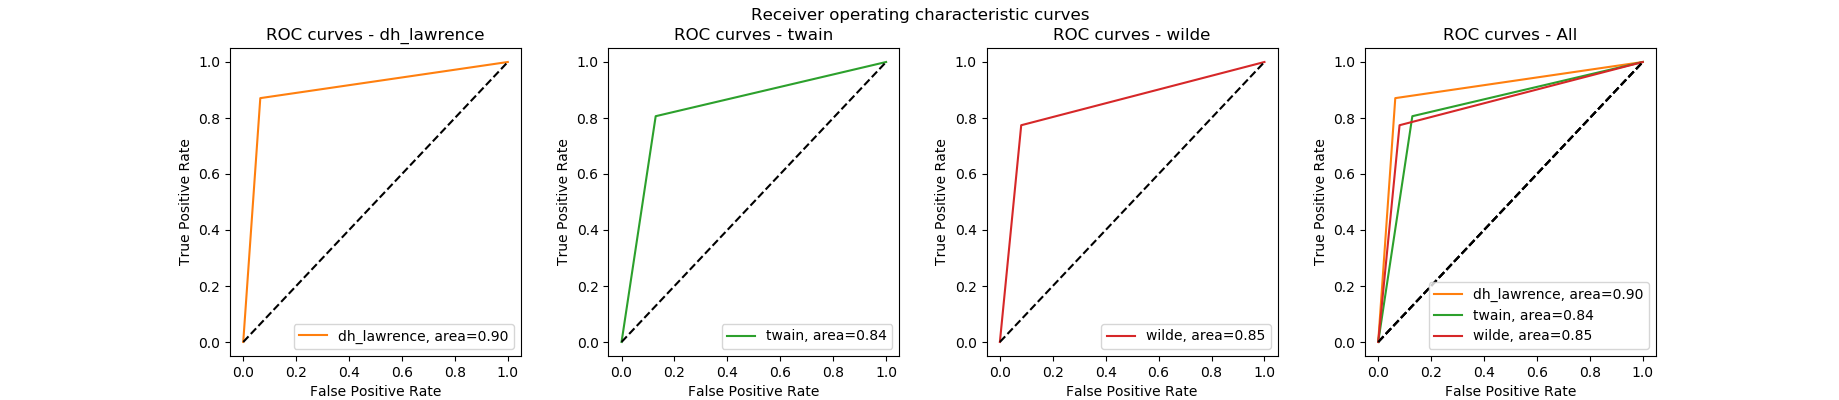
\includegraphics[width=\textwidth]{results_4/authors_ROC.png}
	\caption{ROC CUrves}
\end{figure}
\subsection{Confusion matrices}
\begin{figure}
	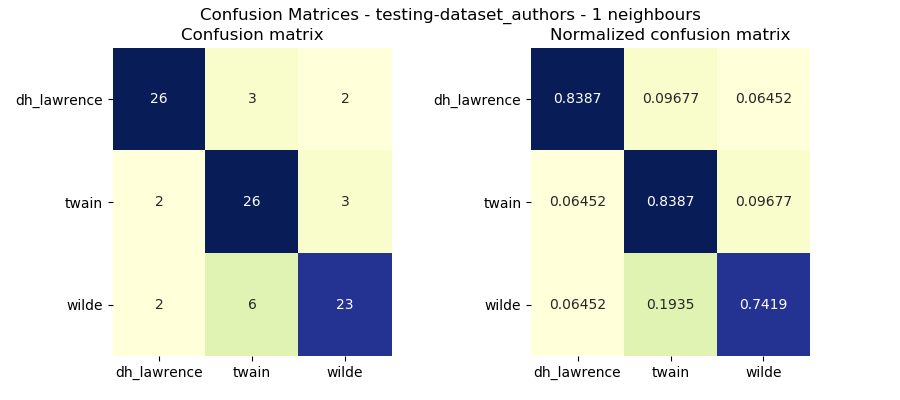
\includegraphics[width=\textwidth]{results_4/authors_Confusion_matrices.png}
	\caption{Confusion matrices for dataset ``authors''}
\end{figure}
\subsection{Truncated SVD reduction}
\begin{figure}
	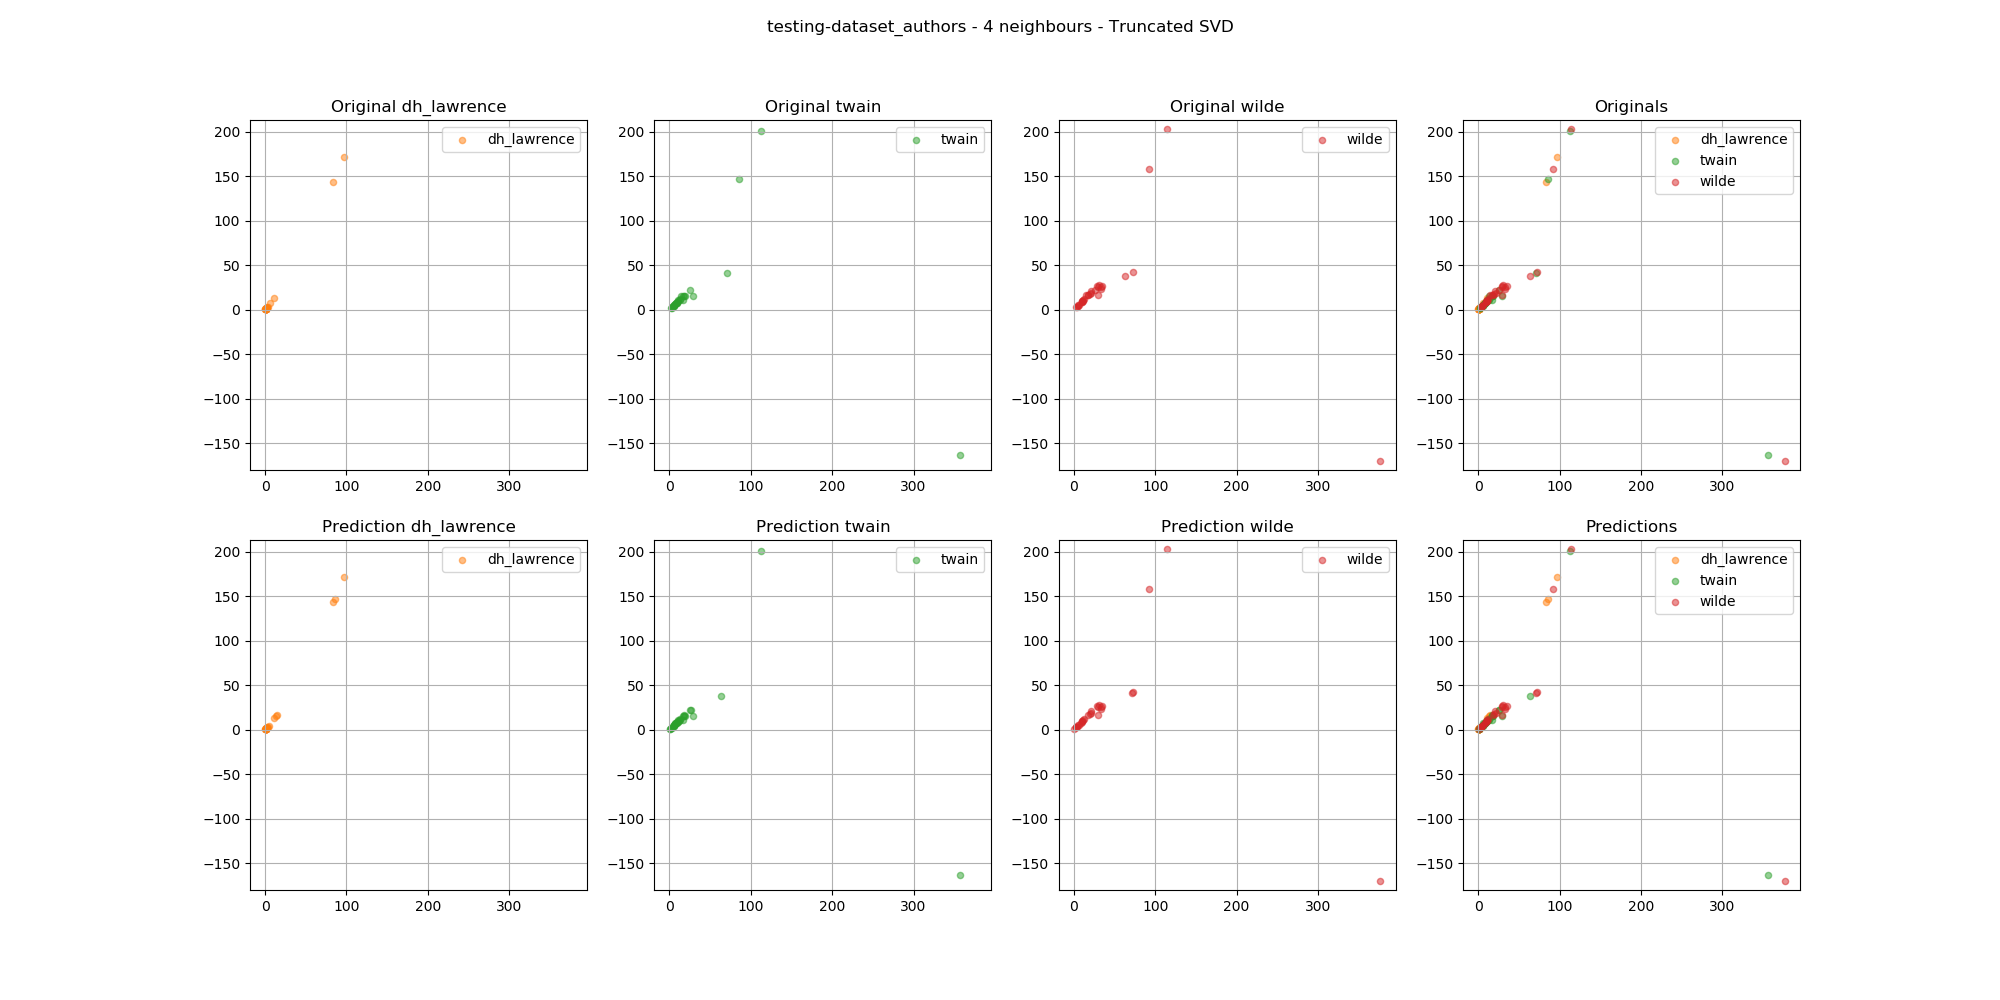
\includegraphics[width=\textwidth]{results_4/authors_Truncated_SVD.png}
	\caption{Dimensionality reduction using truncated SVD in dataset ``authors''}
\end{figure}
\subsection{Most defining word clouds}
\begin{figure}
	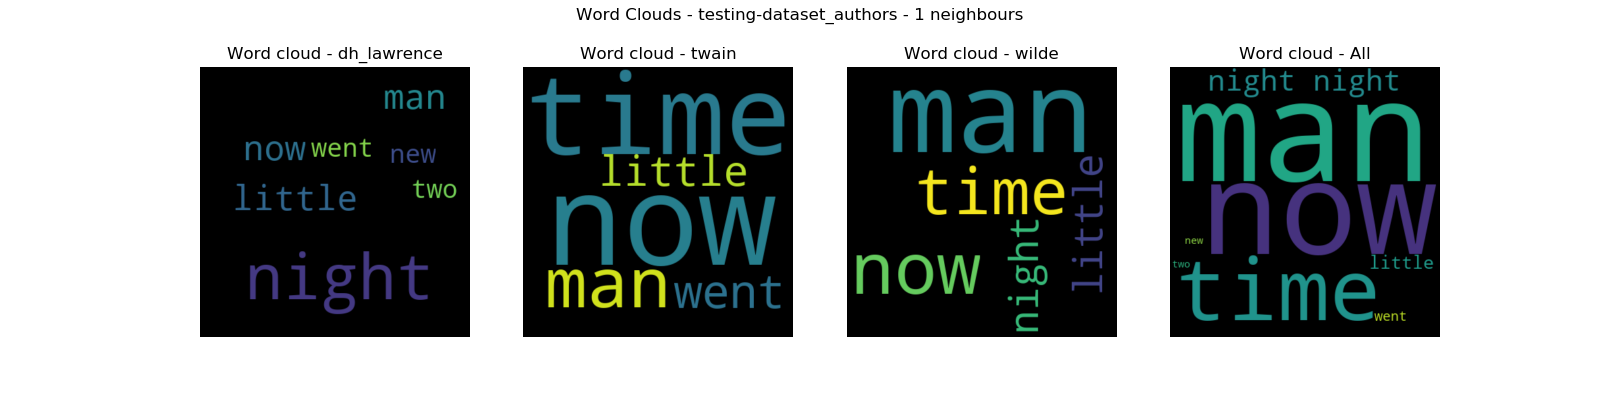
\includegraphics[width=\textwidth]{results_4/authors_Word_Clouds.png}
	\caption{Word clouds}
\end{figure}
\subsection{Representatives points usage}
\begin{figure}
	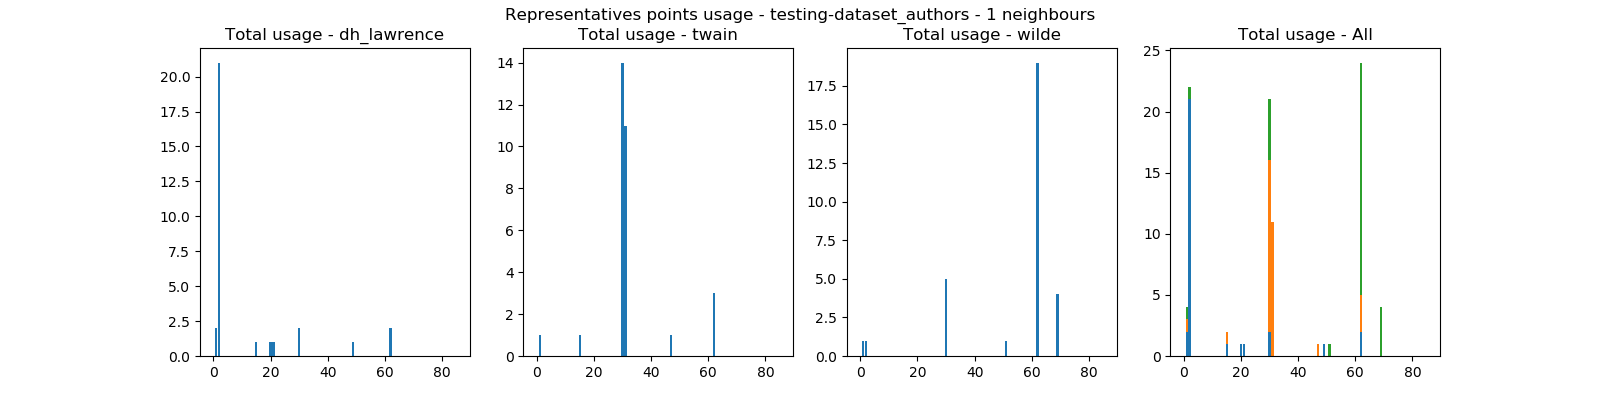
\includegraphics[width=\textwidth]{results_4/authors_Representatives_points_usage.png}
	\caption{Representatives points usage}
\end{figure}

\clearpage
\section{Literary periods}
The ``literary periods'' dataset contains \(1060\) texts from 4 literary periods: Modernism, Realism, Romanticism and Naturalism. Each period has \(265\) documents.
\subsection{Precision varying with neighbors number}
\begin{figure}
	\includegraphics[width=0.4\textwidth]{precision_scores/periods.png}
	\caption{Precision scores}
\end{figure}
\subsection{ROC Curves}
\begin{figure}
	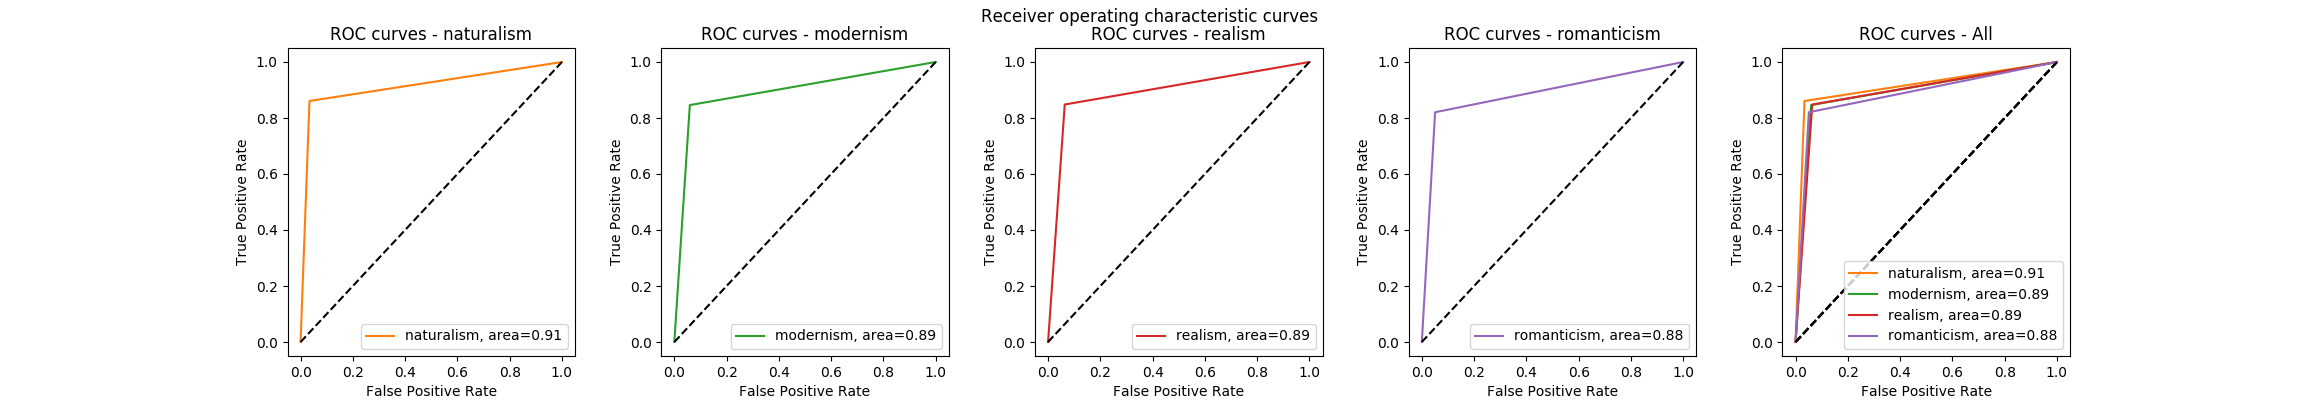
\includegraphics[width=\textwidth]{results_1/periods_ROC.png}
	\caption{ROC CUrves}
\end{figure}
\subsection{Confusion matrices}
\begin{figure}
	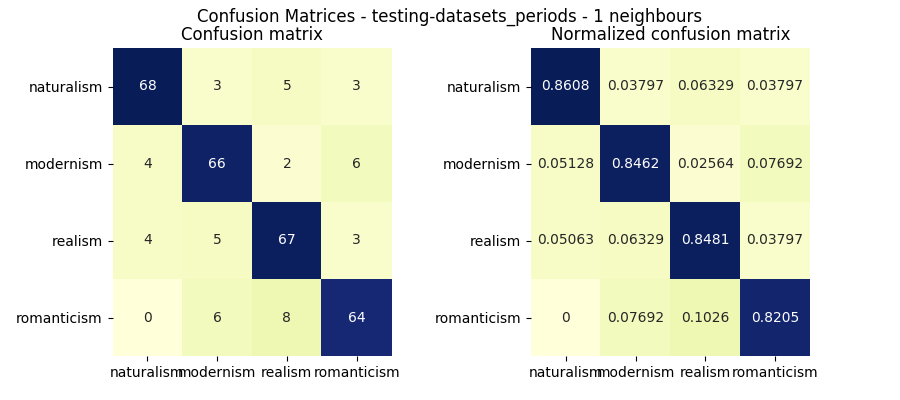
\includegraphics[width=\textwidth]{results_1/periods_Confusion_matrices.png}
	\caption{Confusion matrices for dataset ``periods''}
\end{figure}
\subsection{Truncated SVD reduction}
\begin{figure}
	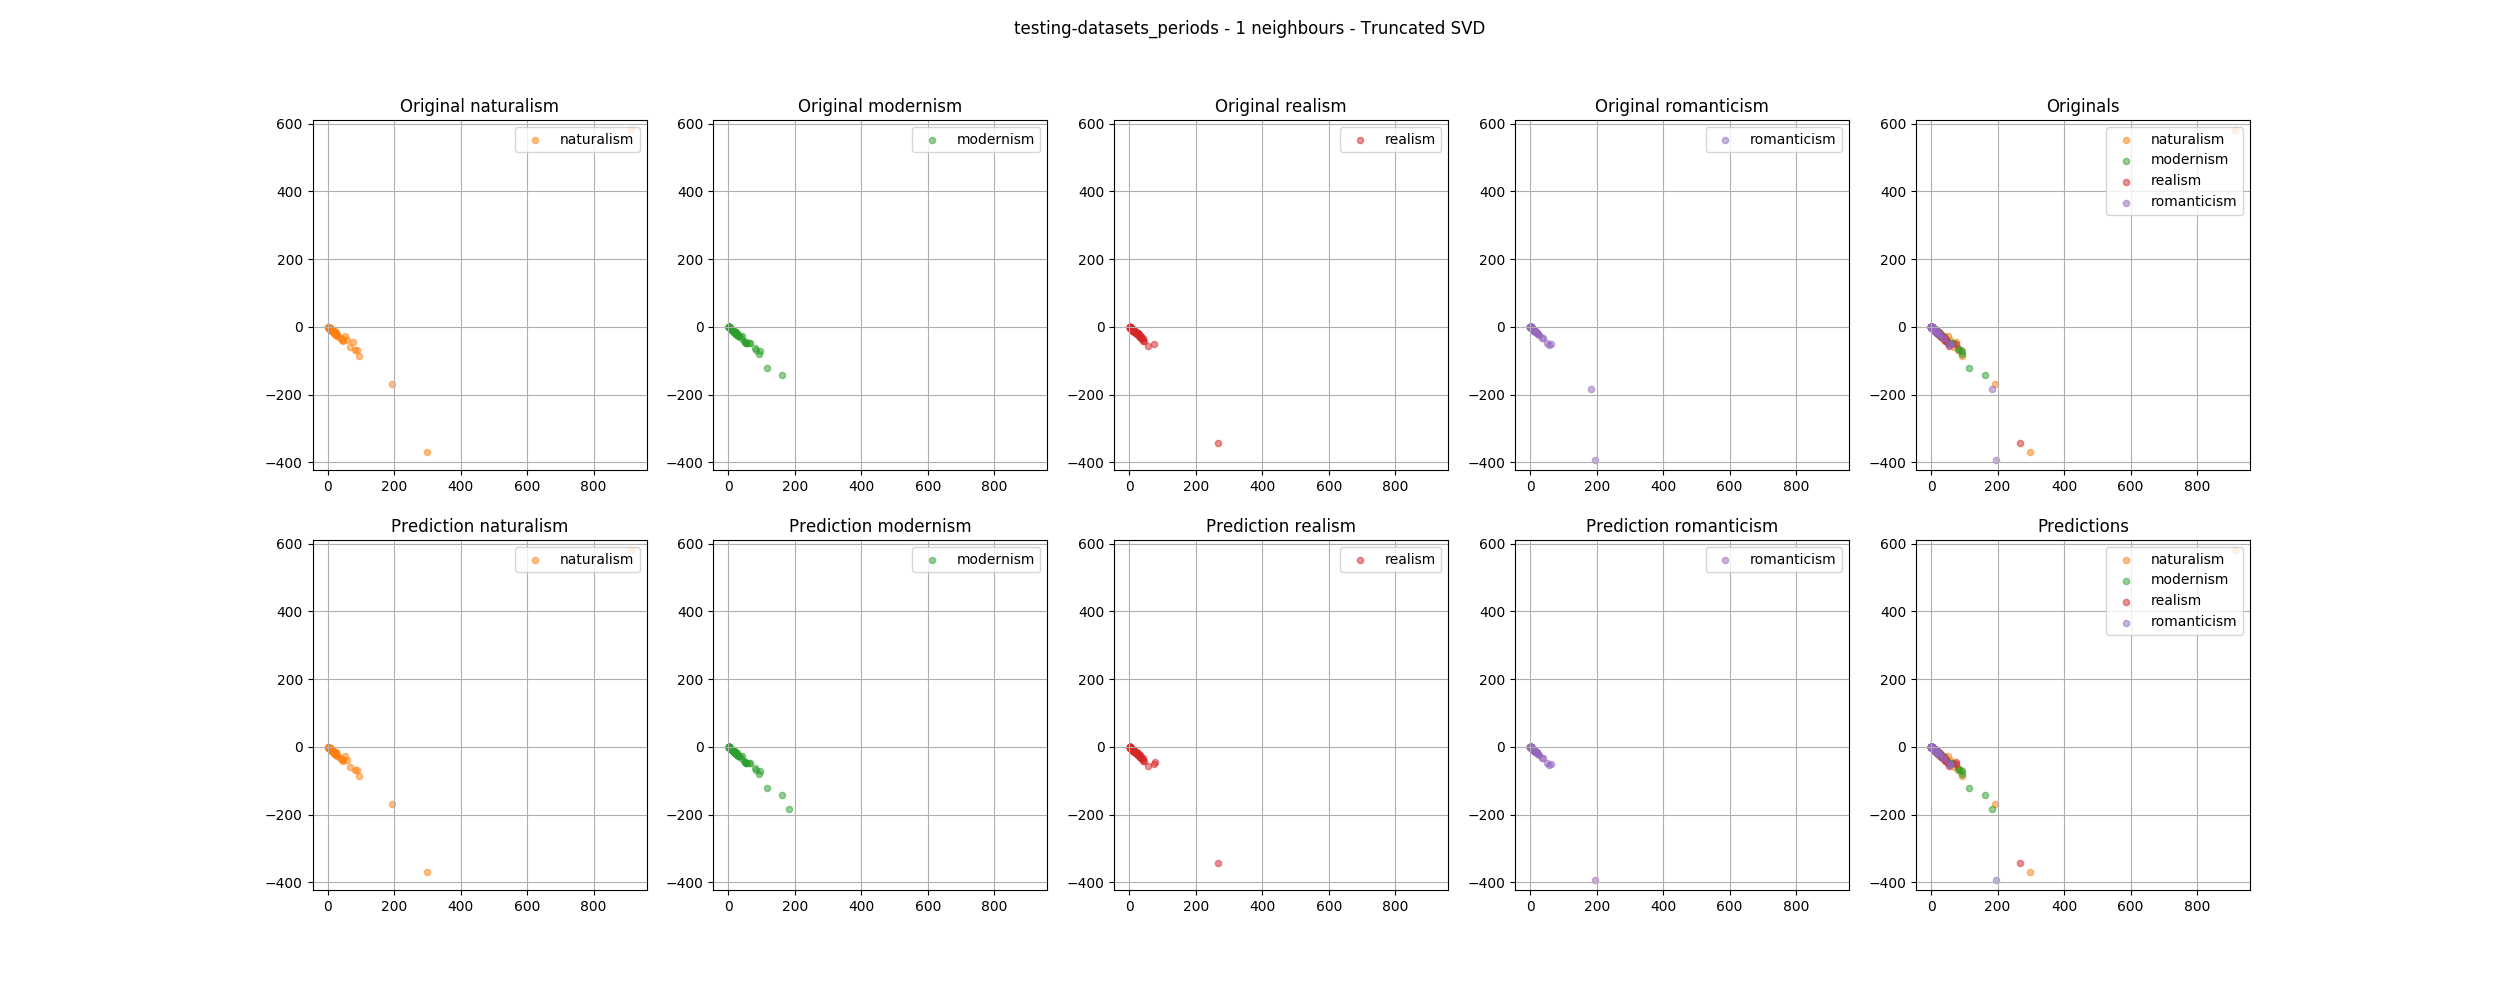
\includegraphics[width=\textwidth]{results_1/periods_Truncated_SVD.png}
	\caption{Dimensionality reduction using truncated SVD in dataset ``periods''}
\end{figure}
\subsection{Most defining word clouds}
\begin{figure}
	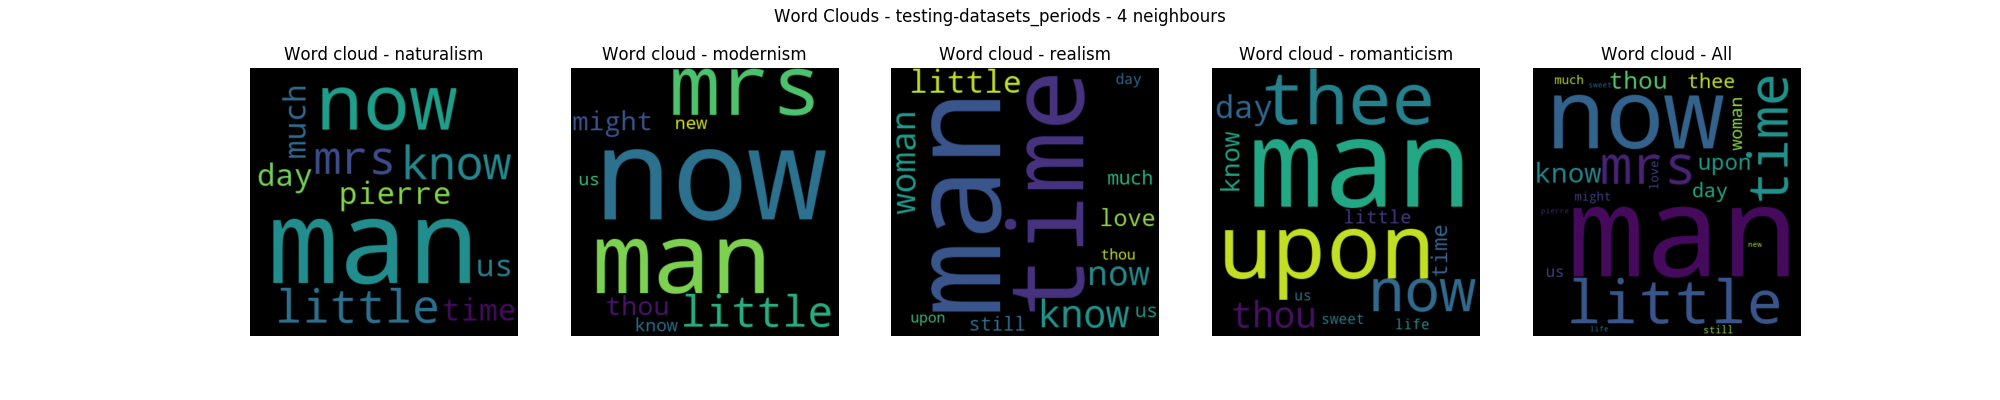
\includegraphics[width=\textwidth]{results_1/periods_Word_Clouds.png}
	\caption{Word clouds}
\end{figure}
\subsection{Representatives points usage}
\begin{figure}
	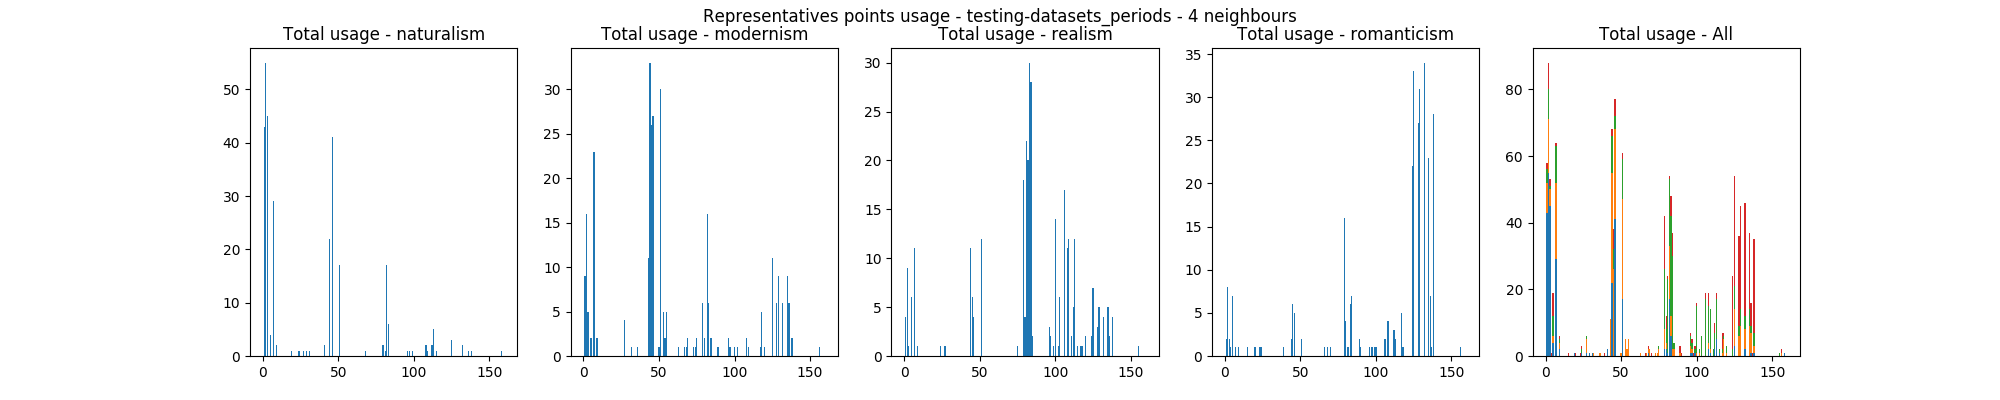
\includegraphics[width=\textwidth]{results_1/periods_Representatives_points_usage.png}
	\caption{Representatives points usage}
\end{figure}

\clearpage
\section{Recipes websites}
The ``recipes websites'' dataset contains \(12768\) texts from 4 Italian websites dedicated to recipes: Misya, Salepepe, Zafferano and Lacucinaitaliana. Every website in the dataset has \(3192\) texts.
\subsection{Precision varying with neighbors number}
\begin{figure}
	\includegraphics[width=0.4\textwidth]{precision_scores/recipes_websites.png}
	\caption{Precision scores}
\end{figure}
\subsection{ROC Curves}
\begin{figure}
	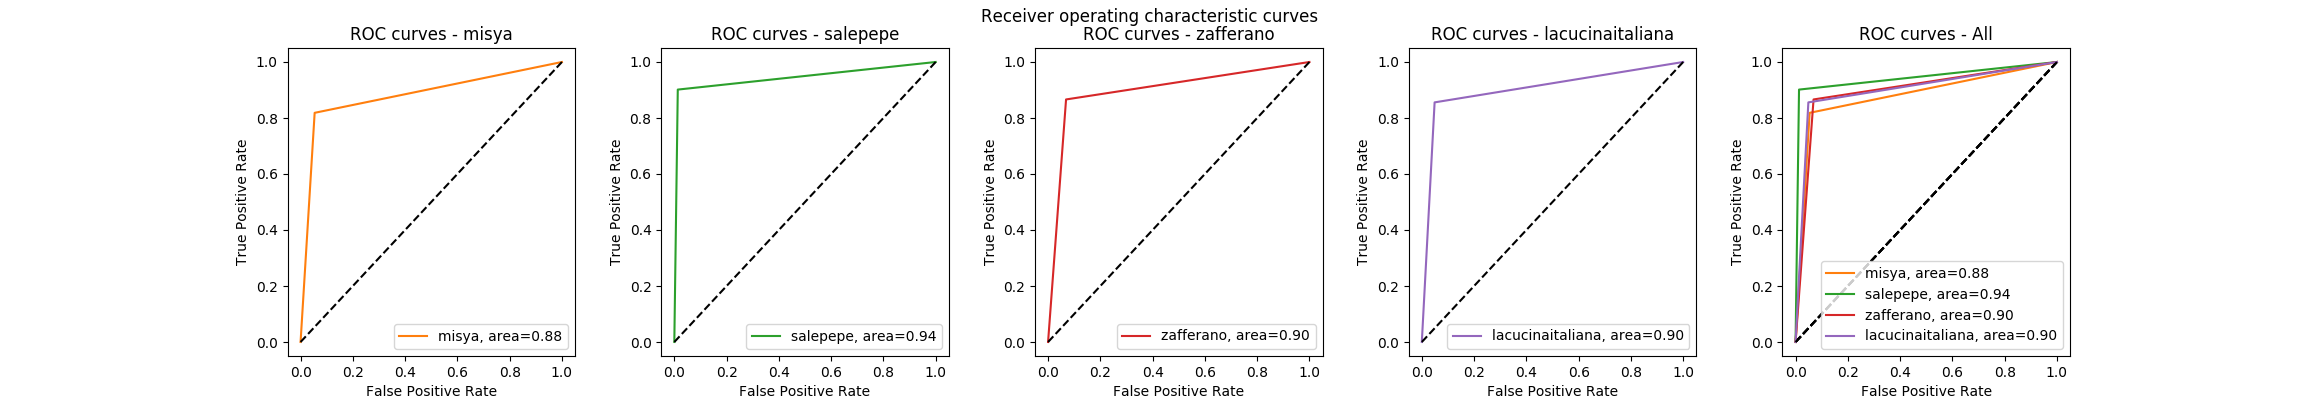
\includegraphics[width=\textwidth]{results_1/recipes_websites_ROC.png}
	\caption{ROC CUrves}
\end{figure}
\subsection{Confusion matrices}
\begin{figure}
	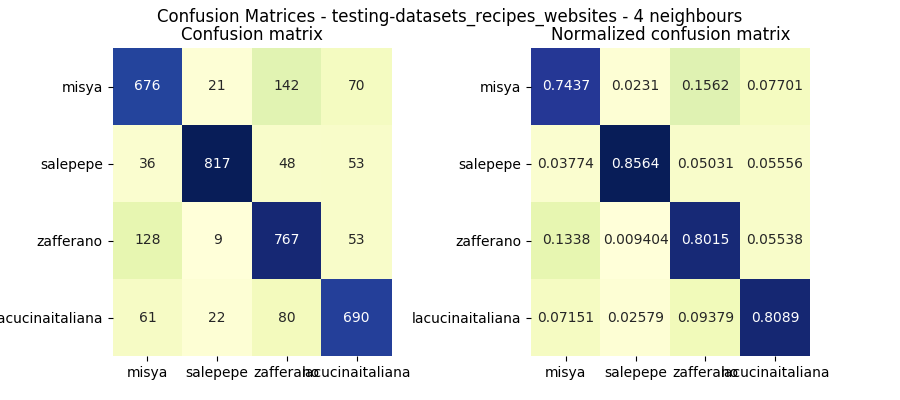
\includegraphics[width=\textwidth]{results_1/recipes_websites_Confusion_matrices.png}
	\caption{Confusion matrices for dataset ``recipes websites''}
\end{figure}
\subsection{Truncated SVD reduction}
\begin{figure}
	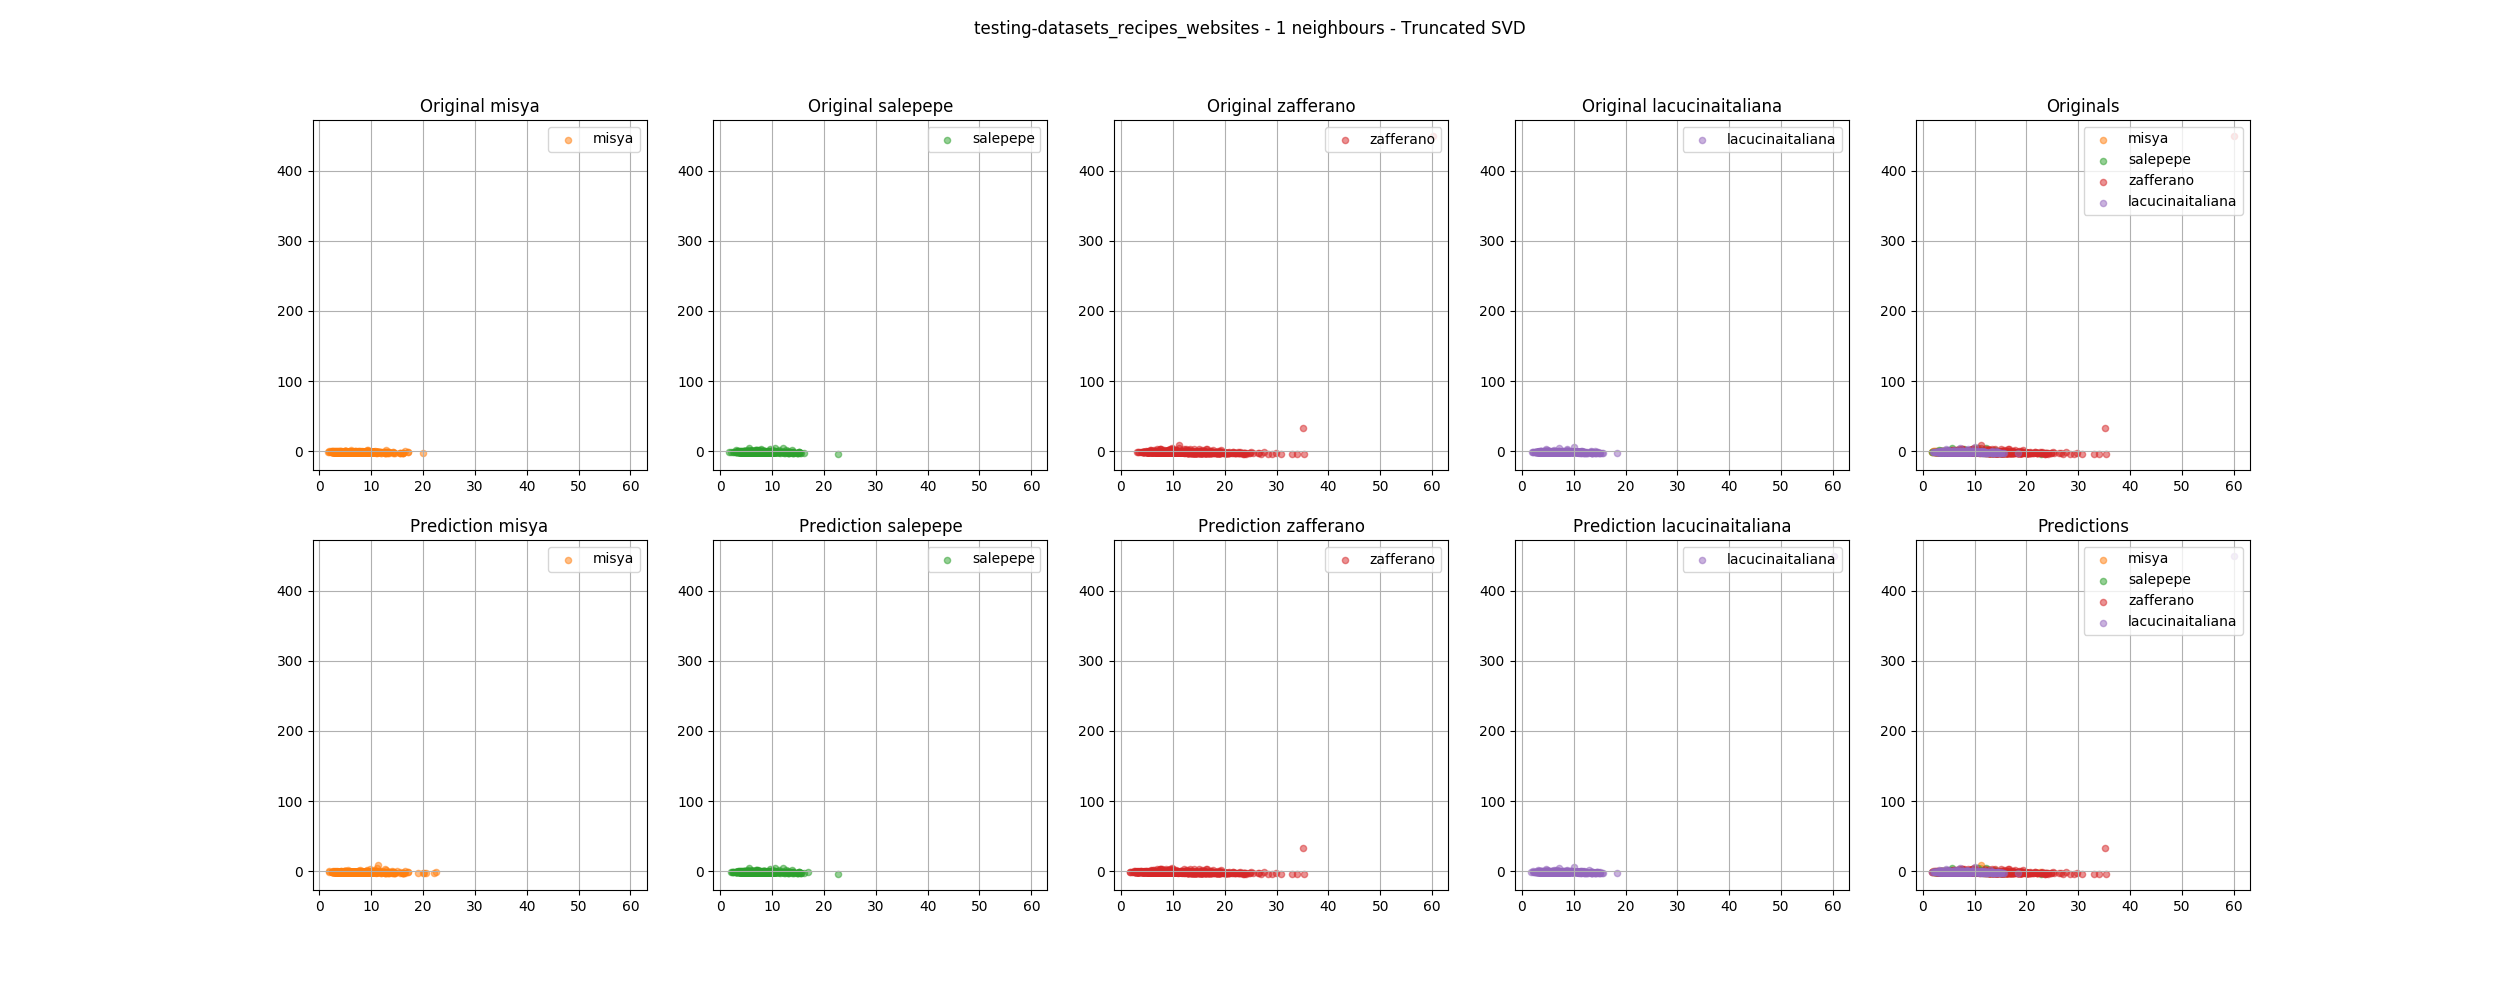
\includegraphics[width=\textwidth]{results_1/recipes_websites_Truncated_SVD.png}
	\caption{Dimensionality reduction using truncated SVD in dataset ``recipes websites''}
\end{figure}
\subsection{Most defining word clouds}
\begin{figure}
	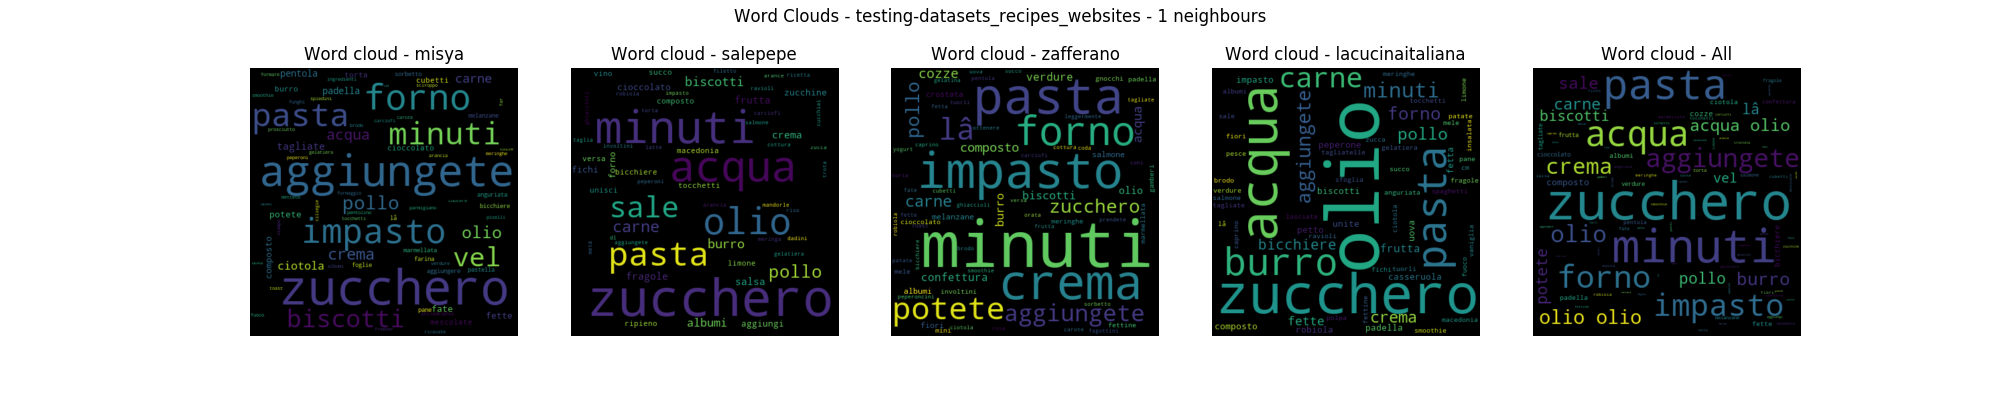
\includegraphics[width=\textwidth]{results_1/recipes_websites_Word_Clouds.png}
	\caption{Word clouds}
\end{figure}
\subsection{Representatives points usage}
\begin{figure}
	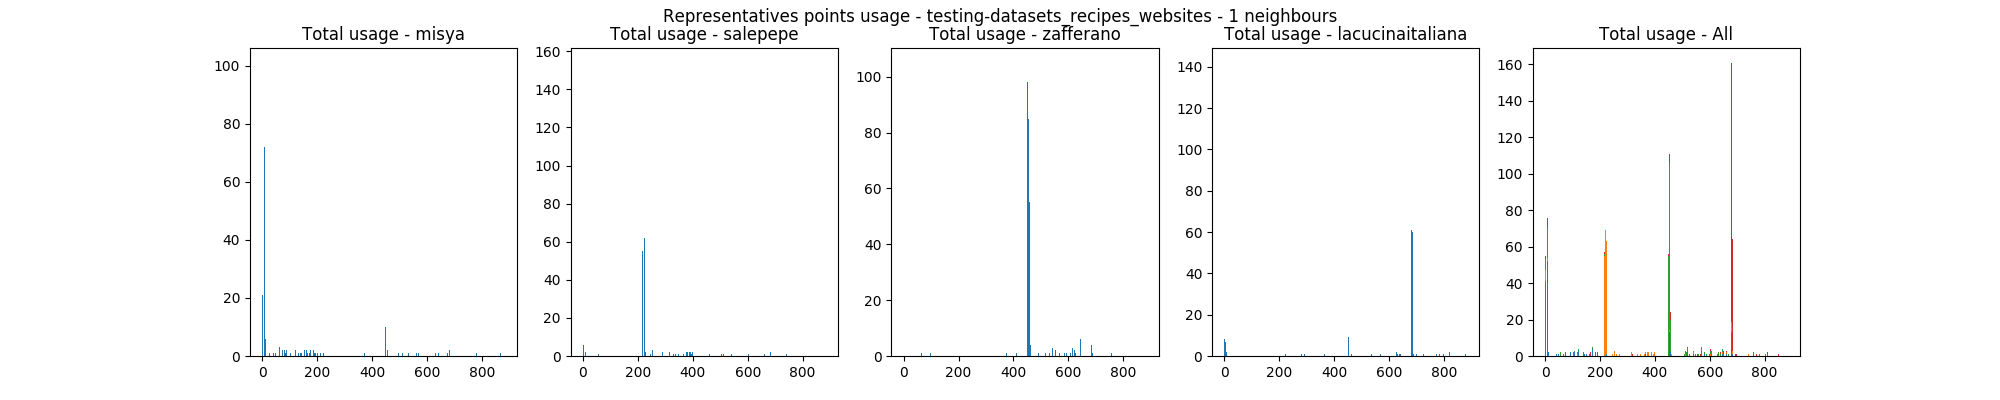
\includegraphics[width=\textwidth]{results_1/recipes_websites_Representatives_points_usage.png}
	\caption{Representatives points usage}
\end{figure}

\clearpage
\section{Newspaper websites}
The ``newspaper websites'' dataset contains \(28000\) texts from 4 italian news websites: Repubblica.it, Moto.it, Scienze.it and Gazzetta.it. Every website in the dataset has \(7000\) texts.
\subsection{Precision varying with neighbors number}
\begin{figure}
	\includegraphics[width=0.4\textwidth]{precision_scores/various_websites.png}
	\caption{Precision scores}
\end{figure}
\subsection{ROC Curves}
\begin{figure}
	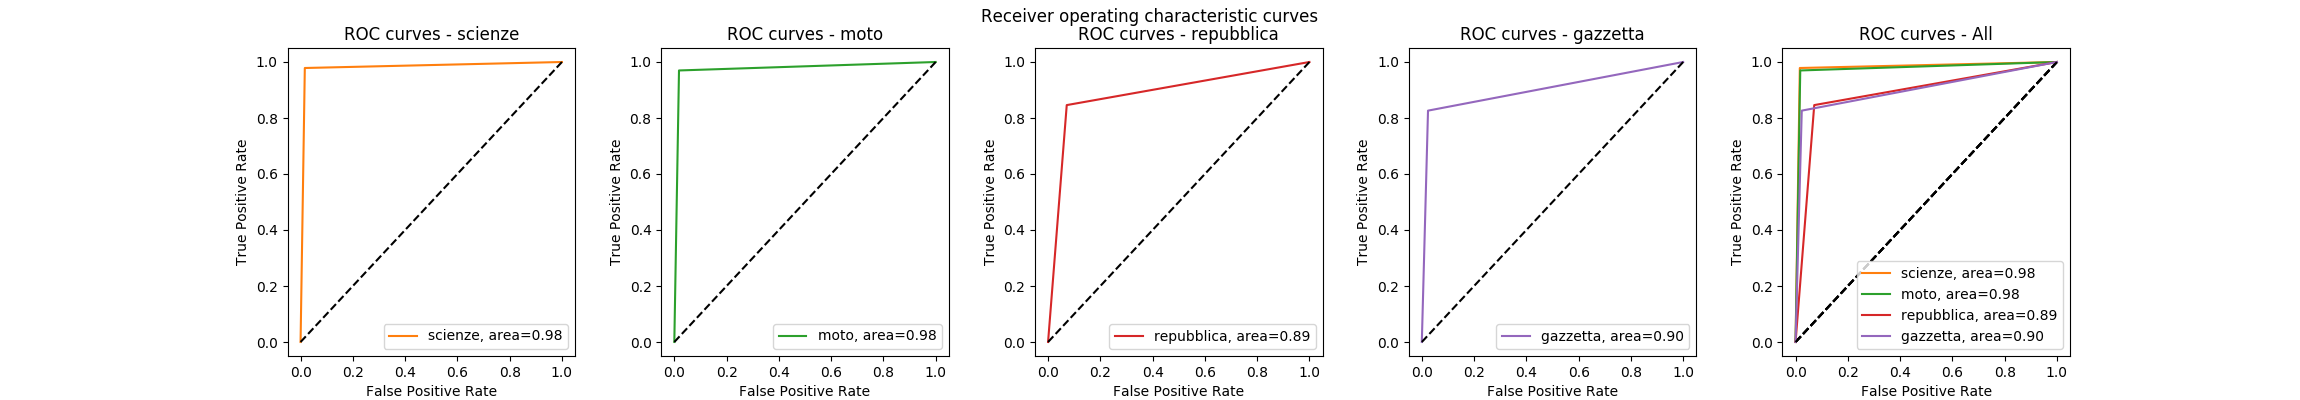
\includegraphics[width=\textwidth]{results_1/various_websites_ROC.png}
	\caption{ROC CUrves}
\end{figure}
\subsection{Confusion matrices}
\begin{figure}
	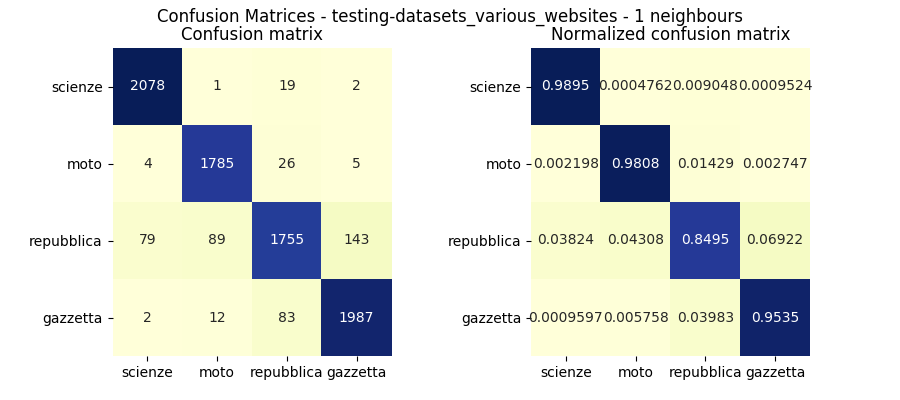
\includegraphics[width=\textwidth]{results_1/various_websites_Confusion_matrices.png}
	\caption{Confusion matrices for dataset ``newspaper websites''}
\end{figure}
\subsection{Truncated SVD reduction}
\begin{figure}
	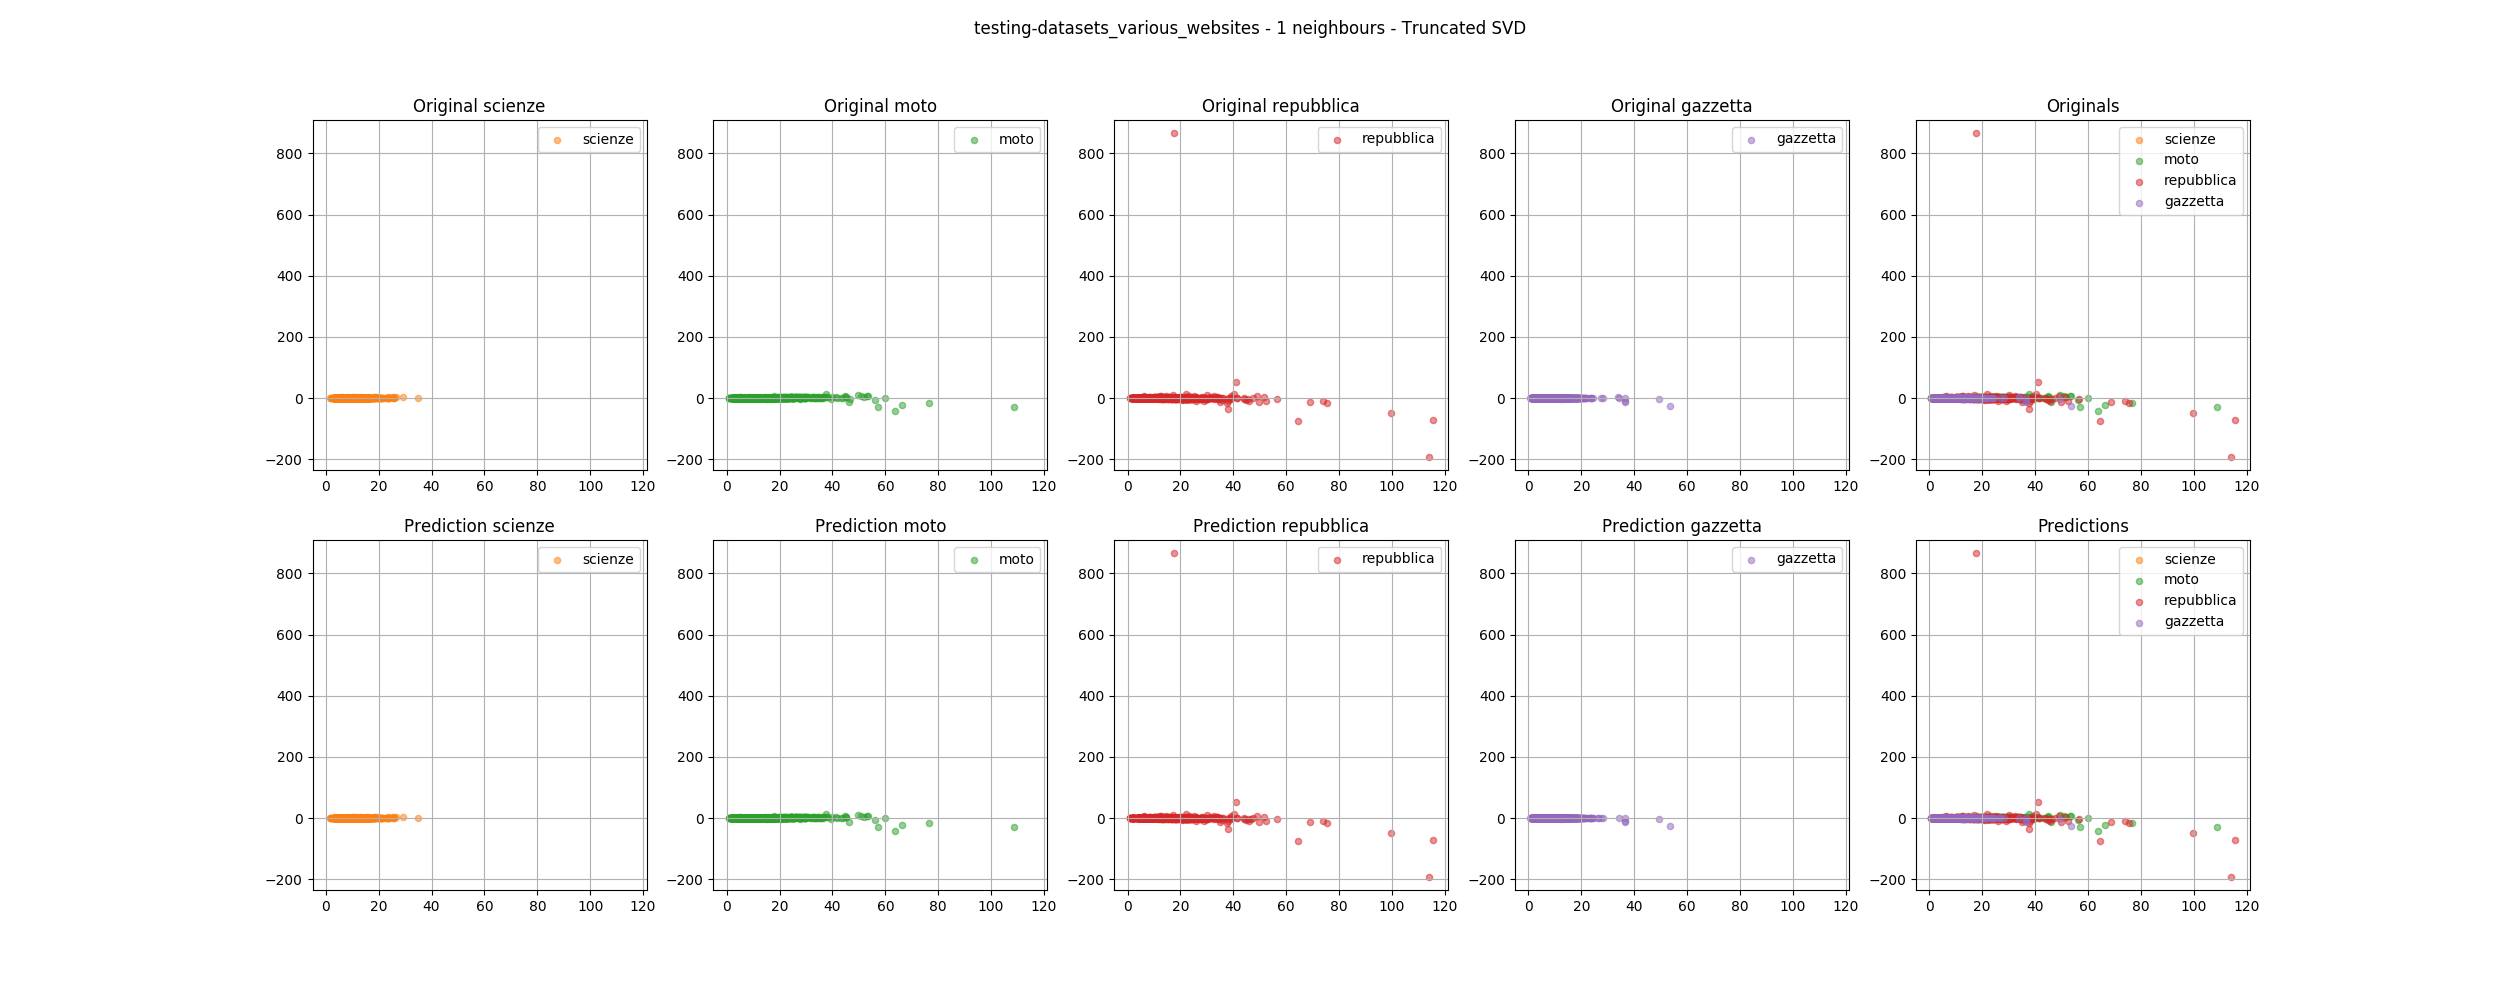
\includegraphics[width=\textwidth]{results_1/various_websites_Truncated_SVD.png}
	\caption{Dimensionality reduction using truncated SVD in dataset ``newspaper websites''}
\end{figure}
\subsection{Most defining word clouds}
\begin{figure}
	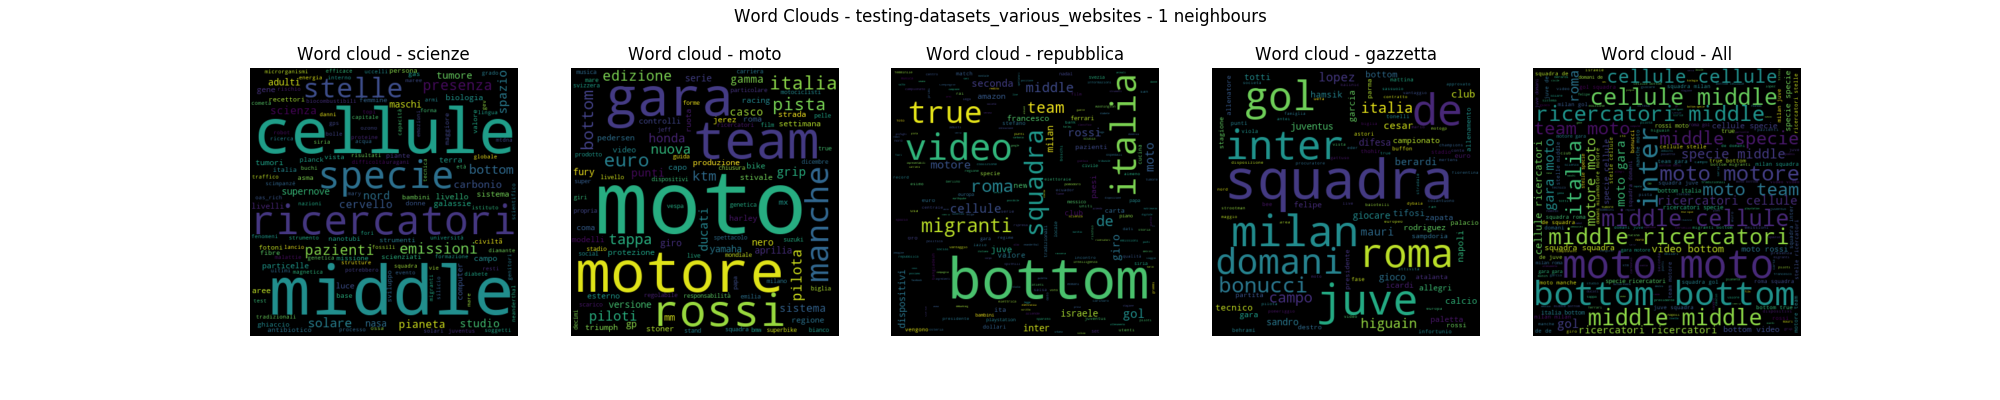
\includegraphics[width=\textwidth]{results_1/various_websites_Word_Clouds.png}
	\caption{Word clouds}
\end{figure}
\subsection{Representatives points usage}
\begin{figure}
	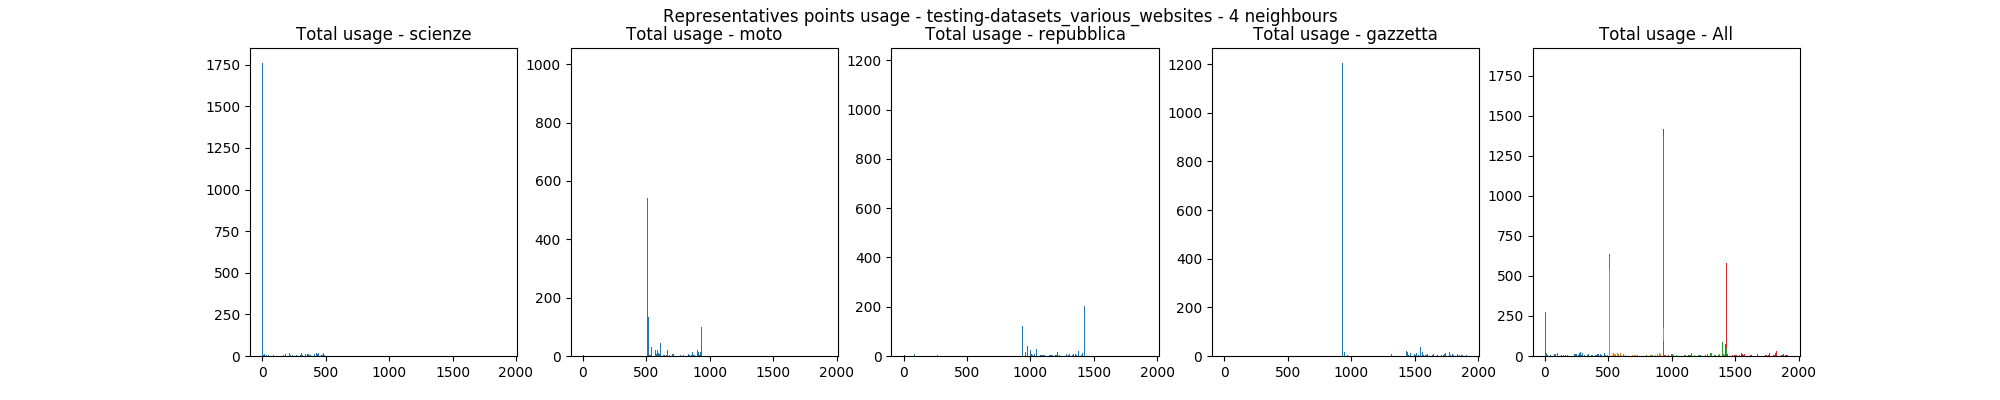
\includegraphics[width=\textwidth]{results_1/various_websites_Representatives_points_usage.png}
	\caption{Representatives points usage}
\end{figure}

\clearpage
\section{Recipes websites or non recipes websites}
This dataset contains \(36000\) texts, with two classes: recipes and non-recipes. Each class has \(18000\) texts.
\subsection{Precision varying with neighbors number}
\begin{figure}
	\includegraphics[width=0.4\textwidth]{precision_scores/recipes.png}
	\caption{Precision scores}
\end{figure}
\subsection{ROC Curves}
\begin{figure}
	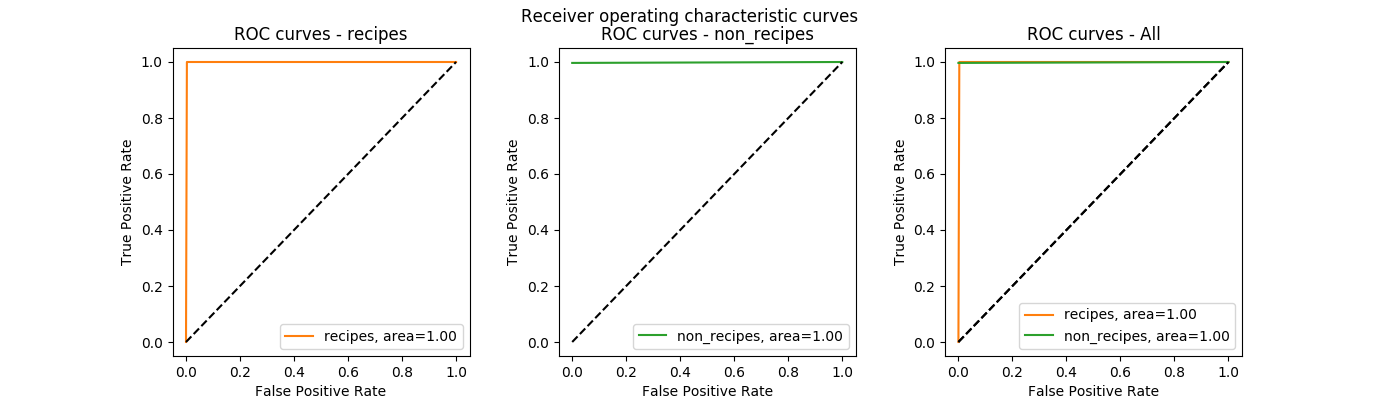
\includegraphics[width=\textwidth]{results_1/recipes_ROC.png}
	\caption{ROC CUrves}
\end{figure}
\subsection{Confusion matrices}
\begin{figure}
	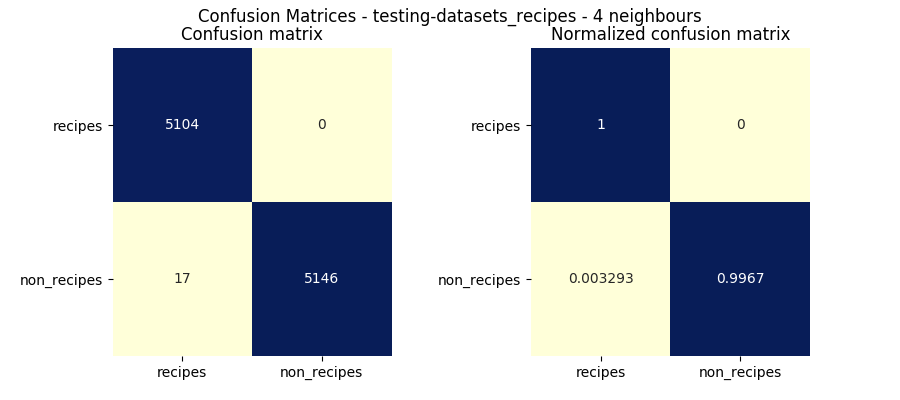
\includegraphics[width=\textwidth]{results_1/recipes_Confusion_matrices.png}
	\caption{Confusion matrices for dataset ``recipes''}
\end{figure}
\subsection{Truncated SVD reduction}
\begin{figure}
	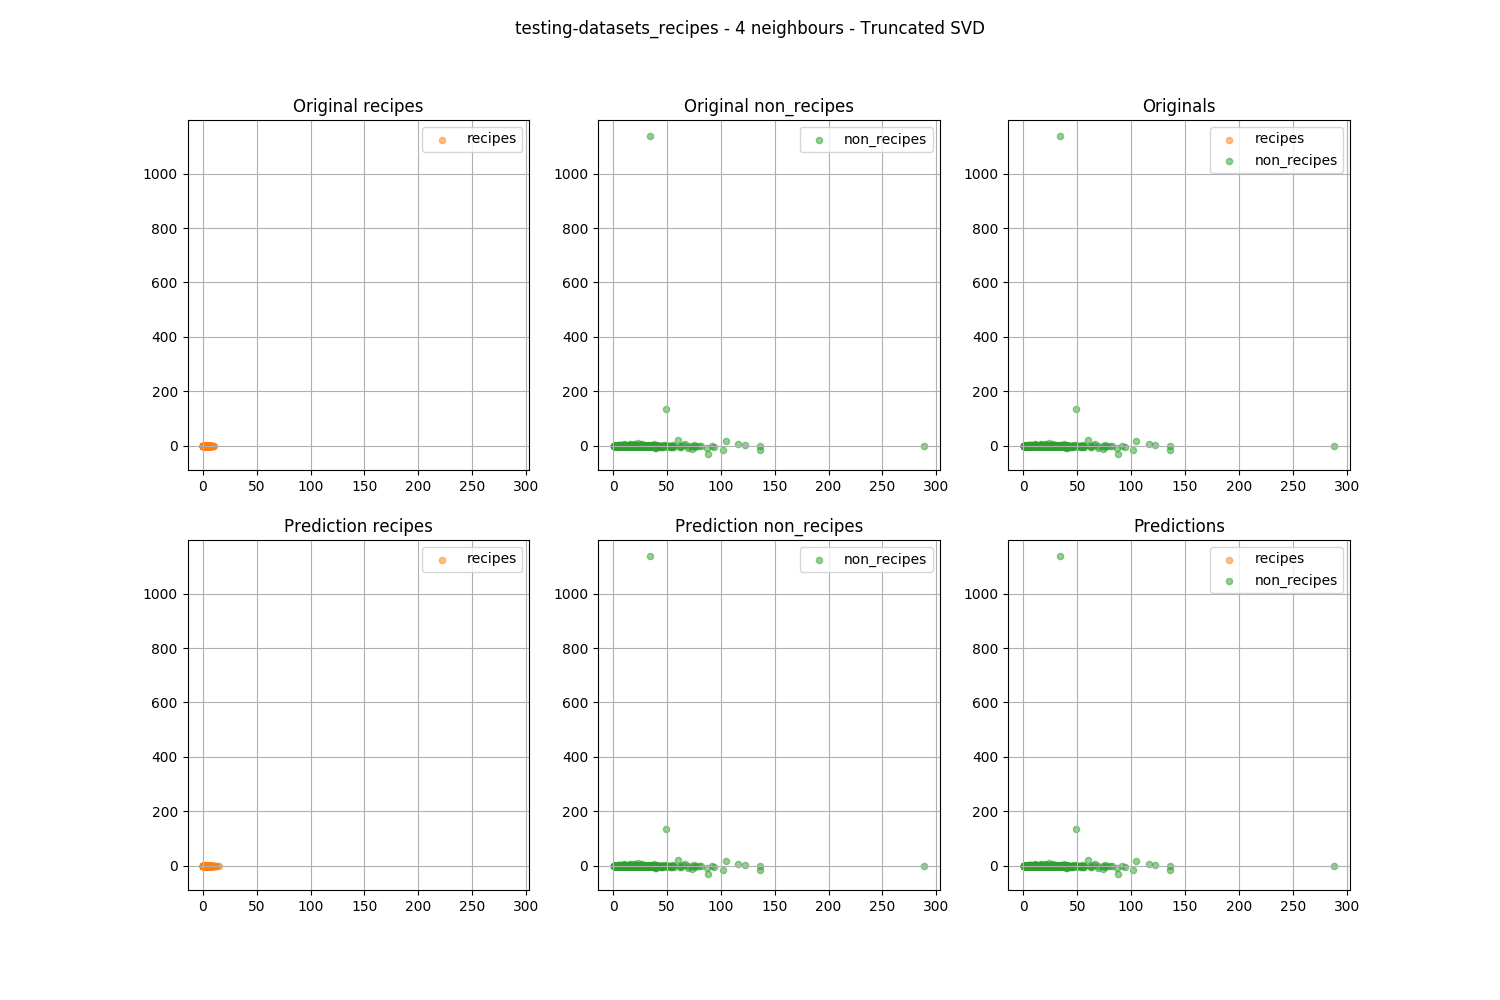
\includegraphics[width=\textwidth]{results_1/recipes_Truncated_SVD.png}
	\caption{Dimensionality reduction using truncated SVD in dataset ``recipes''}
\end{figure}
\subsection{Most defining word clouds}
\begin{figure}
	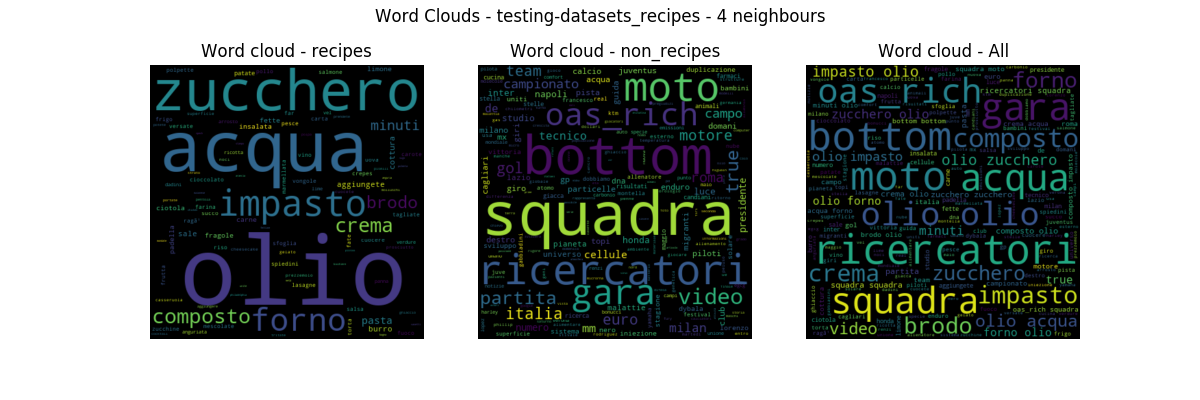
\includegraphics[width=\textwidth]{results_1/recipes_Word_Clouds.png}
	\caption{Word clouds}
\end{figure}
\subsection{Representatives points usage}
\begin{figure}
	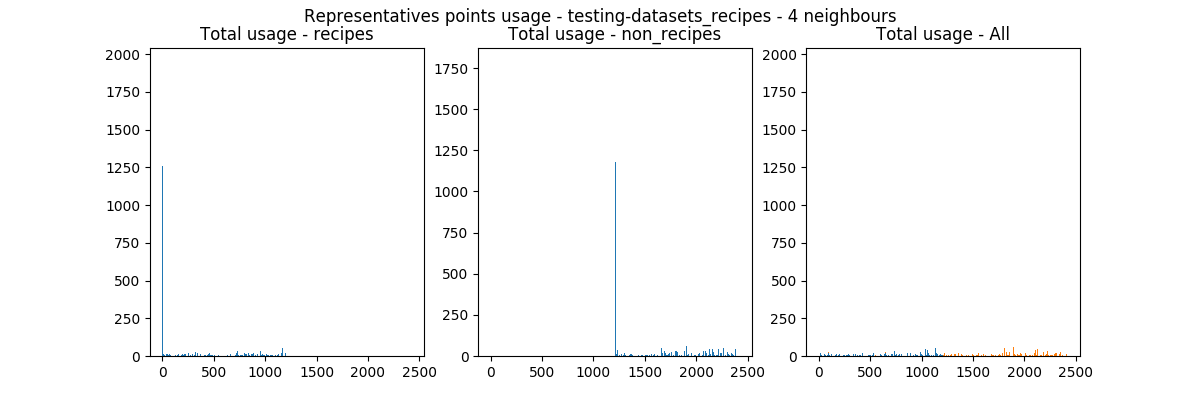
\includegraphics[width=\textwidth]{results_1/recipes_Representatives_points_usage.png}
	\caption{Representatives points usage}
\end{figure}

\clearpage
\section{Nutritional values or non nutritional values}
This dataset contains \(51029\) texts, with two classes: nutritional values and non-nutritional values. The first one has \(5050\) and the second one about ten times as many: \(45979\).
\subsection{Precision varying with neighbors number}
\begin{figure}
	\includegraphics[width=0.4\textwidth]{precision_scores/nutritional_values.png}
	\caption{Precision scores}
\end{figure}
\subsection{ROC Curves}
\begin{figure}
	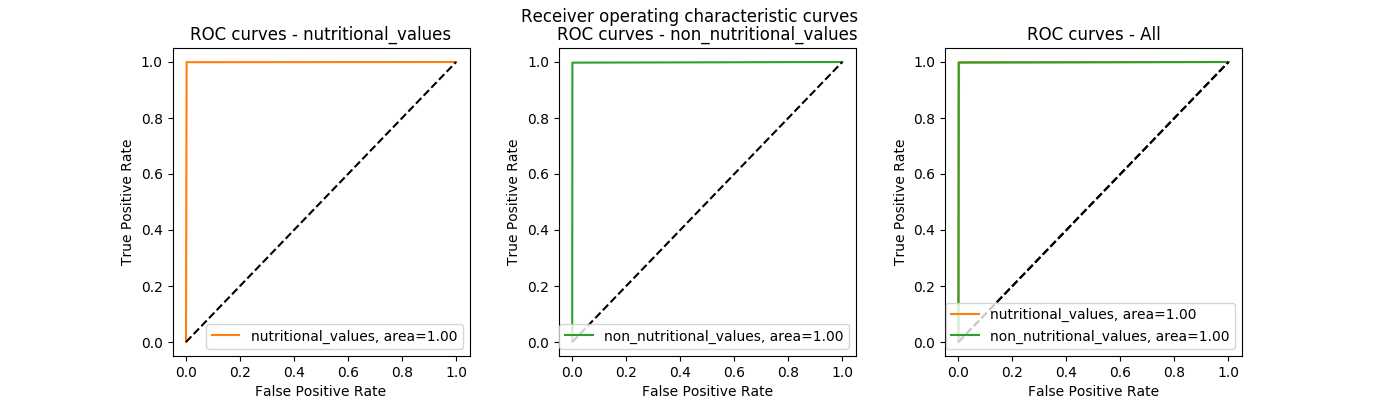
\includegraphics[width=\textwidth]{results_1/nutritional_values_ROC.png}
	\caption{ROC CUrves}
\end{figure}
\subsection{Confusion matrices}
\begin{figure}
	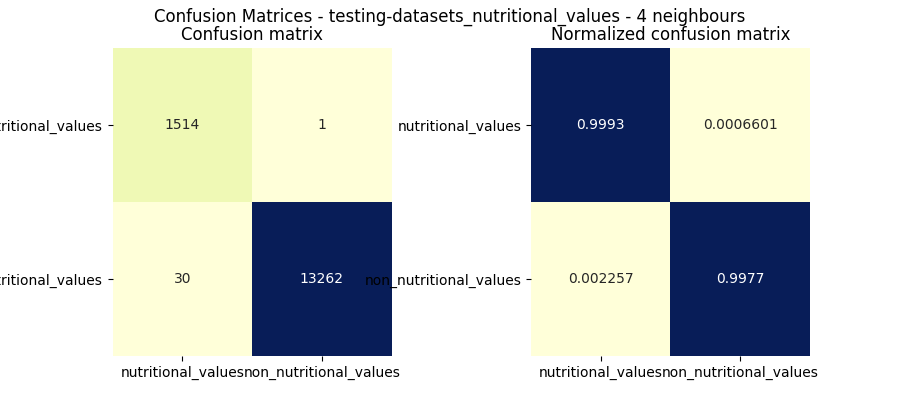
\includegraphics[width=\textwidth]{results_1/nutritional_values_Confusion_matrices.png}
	\caption{Confusion matrices for dataset ``nutritional values''}
\end{figure}
\subsection{Truncated SVD reduction}
\begin{figure}
	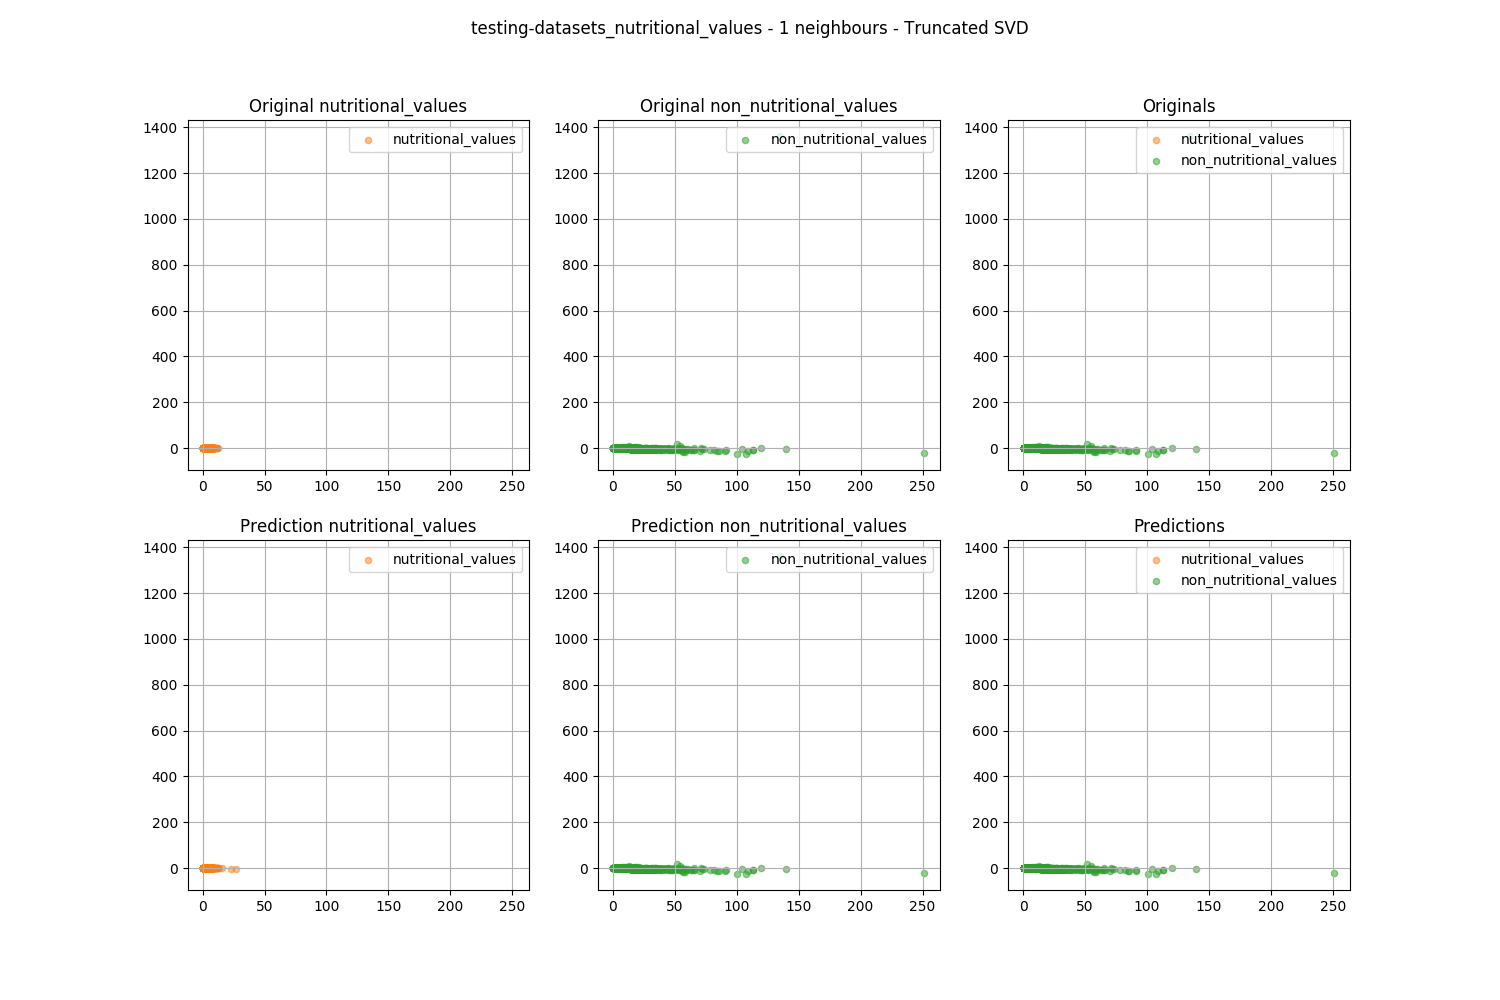
\includegraphics[width=\textwidth]{results_1/nutritional_values_Truncated_SVD.png}
	\caption{Dimensionality reduction using truncated SVD in dataset ``nutritional values''}
\end{figure}
\subsection{Most defining word clouds}
\begin{figure}
	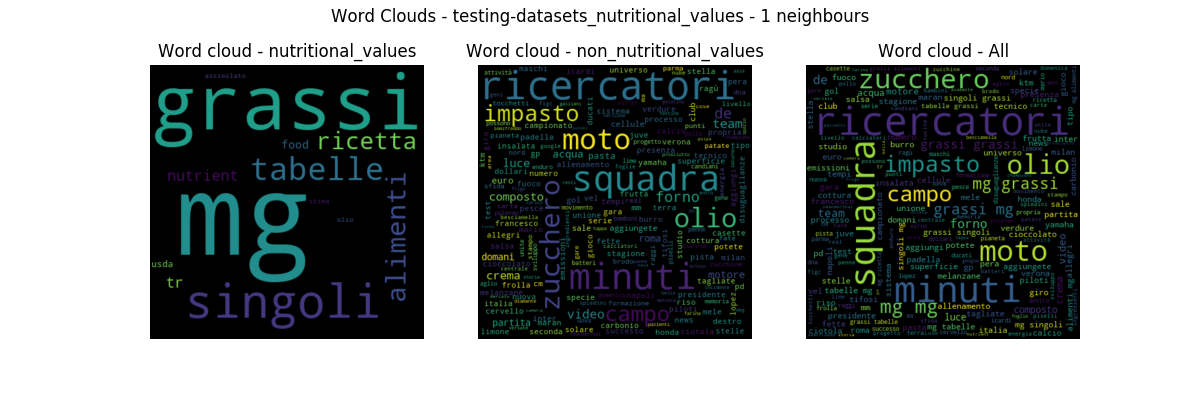
\includegraphics[width=\textwidth]{results_1/nutritional_values_Word_Clouds.png}
	\caption{Word clouds}
\end{figure}
\subsection{Representatives points usage}
\begin{figure}
	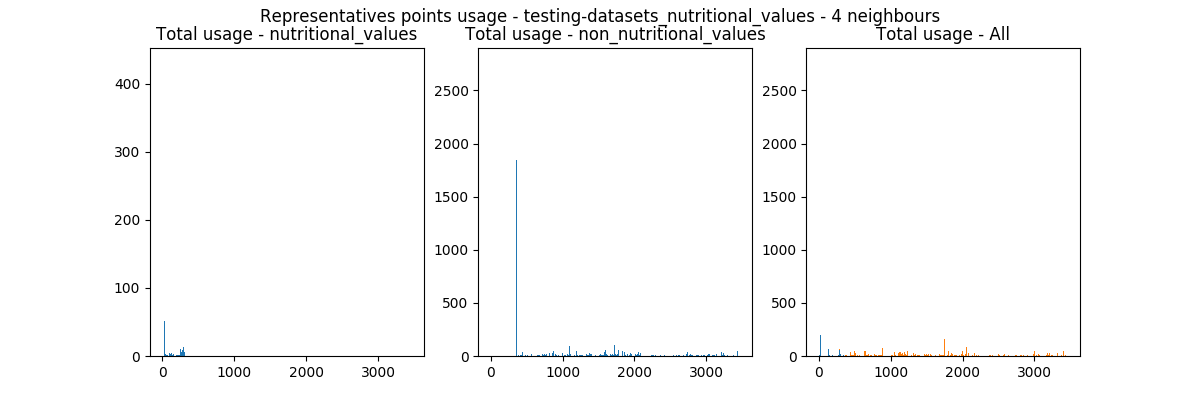
\includegraphics[width=\textwidth]{results_1/nutritional_values_Representatives_points_usage.png}
	\caption{Representatives points usage}
\end{figure}

\end{document}